\documentclass[12pt,letterpaper]{article}
\usepackage{setspace}
\usepackage{cogsci}
\usepackage{pslatex}
\usepackage{apacite}
\usepackage[utf8]{inputenc}
\usepackage{graphicx}
\usepackage[english]{babel}
\usepackage{amsmath}
\usepackage{amsfonts}
\usepackage[colorinlistoftodos]{todonotes}
\usepackage{algorithm}
\usepackage{algpseudocode}
\usepackage[margin=1in]{geometry}

\title{Inverse Structure Learning}
 
\author{{\large \bf Subha Nawer Pushpita},  {\large \bf Riya Arora}\\
\bf \{snpushpi,riya\}@mit.edu}

\setstretch{2.5}
\begin{document}

\maketitle


\section{Abstract}
% abstract will go here - What we were trying to do and why so, basically a combination of Momchil's paper and detecting changes paper
People's sub optimal behavior in predicting or inferring sequential events in a dynamically changing environment has made scientists wonder about human beings' internal noisy mental model structure. In order to study human beings' ability of understanding hidden structure of a dynamically evolving process, we have reproduced partial result from [1] and as a part of that we attempt to model this human behavior through Monte Carlo sampling. We created a normal particle filter as a base line approach. Later we proposed a nested particle filter as a model for human behavior and compared the results of the two particle filters. We have tested the performance of both of these models in unravelling structure of both real agent and synthetic agent and with sufficient evidence, we hypothesized that when normal particle filter has a high similarity score with agent, the nested particle filter will even have higher similarity score with that agent.

\section{Introduction}

% This too will give in detail intro of our goals and stuff, this will basically be a combination of Momchil's intro+detecting changes intro with some modification
In our work, we have reproduced results from [1] where we tried to learn the ability of human observers to predict sequential events in dynamically changing environment. Due to inaccessibility to the entire data set, we were able to reproduce partial results involving only inference task.But also our work significantly deviates from the previous work since we compared the similarity of a normal particle filter and nested particle filter with human inference in a more robust way. The normal particle filter we have implemented in our work was able to generate similar task accuracy of [1] and this we recreated results and thus we reproduced their results and the nested particle filter model which we proposed has provided consistently better results when both models had higher similarity score with human inference.

Previous studies have shown that we can model the way the brain learns the structure of the world by with Bayesian inference using some kind of Monte Carlo sampling. Since these inference algorithms are stochastic, it becomes difficult to investigate the neural basis of structure learning process. Here comes the particle filters are Monte Carlo techniques for the estimation of the hidden state of a dynamically changing system 
and have recently been proposed as a general class of psychological models. Upon each observed stimuli, the particle filter generates a new distribution of particles from the previous distribution by assigning high weight to particles with more consistency with observation and low weight to particles with inconsistent behavior with the observation. They are often considered as a good model of human decision making process because they neither require heavy computation nor a long memory of past observations. Even with these limitations, a particle filter performs surprisingly well and reaches the statistical optimal strategy when run with a sufficiently large number of particles - resulting into approaching full Bayesian Posterior distribution, conditioned on all prior observations.For the similar reason, a particle filter is also able to mimic sub optimal behavior since reducing the number of particles also implies the reduction in prediction or inference task accuracy. 


When faced with a change detection task, a human being often performs sub optimally because reliable change detection requires accurate interpretation of sequential dependencies in the observed data and several research on decision making has showed human being's inability to correctly interpret sequential events but we want to explain this phenomena and investigate brain's ability to construct the internal mental models of hidden generative structure of the environment. This is where experimentation with a changing environment and human behavior in response to that comes in. 


Using data collected from a simple change detection environment from the experiment set up mentioned [1], we revealed how human subjects perform compared to a normal particle filter model and how we can tune hyper parameters of a particle filter to get task accuracy as close as possible to human beings. This is the part we reproduced from paper, but later we gave more robust comparisons of both models - normal particle filter and our proposed nested particle filter with human inferences. Whereas the approach in the aforementioned paper focuses on comparing human similarity with models in terms of task accuracy, or in other words, how close the task accuracies are from both the model and the human, we took one step further and compared straight the model inferences with human inferences for a given task and calculated similarity score based on how many times the model inferred the same state as the human being. 

Apart from normal particle filter, we have proposed nested particle filter model where upon each observed stimuli, each particle filter in the nested particle filter gets updated(re weight and re sample) following the algorithm of normal particle filter, but each particle filter itself also has a weight and that depends on consistency with the inference of the agent and particle filters with more consistency with the agent(human or synthetic approach in our case) were assigned higher weights and particle filters with lower consistency with the agent inferences were assigned lower weights and then we do the "re sampling of particle filters" themselves, analogous to normal particle filter's "re sampling of particles".

Normal particle filters are a great way to track the state of a
dynamic system for we have a Bayesian model. So if we
have a model of how the system changes in time, possibly in response to inputs, and a model of what observations you should see in particular states, we can use particle filters to track our belief state. But we also observed a possible weakness of this approach. Though we can tune the hyper parameters so that we can get desired optimal/sub optimal/ conditionally optimal behavior, it is also true that the particle filter approaches on its own based on the observations we are giving it. In other words, it doesn't get affected by the agent's actions or inferences at any given time, because the particle re weight or sampling entirely depends on the consistency of observation with the particle. That is why unless a human subject's possible model for inferring hidden structure of the world is a particle filter, it is less likely that we will be completely be able to uncover the model humans use in their mind.

This is where nested particle filter comes in, because a nested particle filter consists of multiple particle filters and each particle filter's particles gets updated based on the observation but each particle filter also has its own importance weight and a particle filter with more consistency with agent's inference is weighted higher and a particle filter with less consistency with agent inference is assigned lower weight in each trial. This is how we tried to mimic agent's behavior through a nested particle filter model.


We have later evaluated our proposed nested particle filter scheme on synthetic data and showed that in uncovers structure inferred by the agent with a very high accuracy, and with significantly higher accuracy than normal particle filter. We evaluated both of these models on real human data and hypothesized that individuals who have a good similarity score (above 0.6) with normal particle filter, they even tend to have a better similarity score with nested particle filter, implying that mindful observers are more likely to be aligned with nested particle filter. We also discussed the future scopes of our work and plausible modifications of experiment set up, model and hyper parameter tuning in order to fit human data more effectively. 

\section{Particle Filter}
%3 subsections will go here
% I will do this part, a detailed explanation of particle filter and algorithm 1, the algorithm of particle filter 
% Add the PF diagram from detecting changes paper and give them credit 
Particle filters or Sequential Monte Carlo (SMC) methods are a set of Monte Carlo algorithms used to solve filtering problems arising in Bayesian statistical inference. In the theory of stochastic processes, the filtering problem is a mathematical model for a number of state estimation problems in signal processing and related fields.The general idea is to establish a "best estimate" for the true value of some system from an incomplete, potentially noisy set of observations on a dynamic system. 

Particle filtering uses a set of particles (also called samples) to represent the posterior distribution of some stochastic process given noisy and/or partial observations and this distribution is updated after each observation and those particles with more consistency are assigned higher weight and those with inconsistency with the observation are penalized and assigned low weights. Particle filter techniques provide a well-established methodology for generating samples from the required distribution without requiring assumptions about the state-space model or the state distributions. For our work in this project, we have used sequential importance re sampling in particle filter. The particle filter algorithm which we used in our implementation is attached as algorithm $1$ in the Appendix section.

\section{Sequential Importance Resampling}
Sequential importance Resampling (SIR) approximates the filtering probability density ${p(x_{k}|y_{0},\cdots ,y_{k})}$ by a weighted set of N samples ${\displaystyle \left\{\left(w_{k}^{(i)},x_{k}^{(i)}\right)\ :\ i\in \{1,\cdots ,N\}\right\}.}$ The importance weights ${\displaystyle w_{k}^{(i)}}$ are approximations to the relative posterior probabilities (or densities) of the samples such that
${\sum _{i=1}^{N}w_{k}^{(i)}=1.}$ On a higher level,we sample N times from the set of particles and the probability of drawing each particle is given by its importance weight and more particles/computation are focused on the states
with high probability mass
\section{Nested Particle Filter}
% 2 subsections will go here 
% I will do this part too, a detailed exp of nested PF and algorithm 2, the algorithm of nested PF
We are introducing a particle filtering method for more effectively capturing human behavior. As pretty explanatory from the name, a nested particle filter consists of multiple particle filters and each particle in a particle filter gets updated based on the observation at time $t$ and the particles with more consistency with the observation get higher weight, but each particle filter itself is also reweighed after each human inference and the particle filters with more consistency with agent inference get higher weight whereas the particle filters with low consistency with agent inference gets penalized. The Nested particle filter algorithm we proposed is attached in the appendix section. 
\section{Method}
% [Riya] Give a detailed description of the human dataset we used (if you use a part of it, then explain that part and may be refer to the fact that this was adopted from that paper, but explain the dataset description nonetheless in detail and how you created those dots or whatever, may be follow the change detection paper, we will put the grey dots graph here or refer to the fact where in appendix those graphs are, because this is the part we reproduced and not like our original contribution(even tho we didn't use the same PF algo) and hence shouldn't go to the results I believe and shpuld stay in methods, also explain how you generate human similarity graphs with human data in one or two data, not the results or explanations in this section, results and explanations will go to the next section

We reproduced partial results from Predicting and Detecting Changes. Specifically, we reproduced Figure 4 and the inference part of Figure 7 from Predicting and Detecting Changes. We would have attempted to reproduce the prediction part of Figure 7 also, but we were not given the prediction data from the authors of that paper, they only provided us with their inference data.

Here is the general setup of the experiment. There are 4 pipes, called A, B, C, and D. This pipes are located at positions 0.2, 0.4, 0.6, and 0.8 respectively. Objects are then dropped from pipes. A object dropped from a pipe at location x may not hit the ground at position x. Specifically, where it will hit the ground can be modeled as a normal distribution where sigma = 0.1 and mu = x (the position it was dropped from). The first pipe we pick for an object to be dropped from is random. For all future pipes, the pipe stays the same as the previous pipe most of the time, and occasionally it changes. The task that the humans have is given the location the object drops to, guess the pipe the object dropped from. So the idea behind the algorithm for generating data is that for every trial, it calculates the original pipe and the location the object falls in. The original pipe of the first trial is a random pipe. For every future trial, the pipe the objects falls from is the same as the previous pipe with probability 1-alpha and changes with probability alpha. For every trial, the observed location is a normal distribution with sigma = 0.1 and mu = the location of the pipe the object was dropped from. The implementation of this algorithm is shown in algorithm 4 in the appendix.That is the essence of the experiment.

Here are some more details that the humans are not given. The pipe the object is dropped from will change with probability alpha. Since people aren't told this, the goal of the  experiment is to show that people are more likely to think the pipe will change after a bunch of objects they think fall from the same pipe. For example, if there are 10 objects that a subject thinks falls from pipe A, they are more likely to think that future pipes are not A that if there were only 2 such objects. In our particle filters and in the paper Detecting and Predicting Changes, we model a person's assumed value of alpha as $\alpha = 1-e^{-rk}$ where k is the number of consecutive objects that fell from the same pipe and r is a value that we vary and test different value of.

Here is how we reproduced the results in Figure 4 from Detecting And Predicting Changes. There are two types of dots there, grey dots and black dots. Grey dots is what our model predicts and black dots is what humans respond with. To produce the black dots, we asked the paper authors for their data. We then went through each test block for every person. For each of these blocks, we have one dot. To plot this dot, we calculated their accuracy and the proportion of response changes. We then estimated the value of alpha for each block by calculating the proportion of pipe changes and seeing if this proportion is closer to 0.08, 0.16, or 0.32. While this may or may not be the actual value of alpha, we believe that this will be correct most of the time, and this is the best method for estimating alpha. We then graphed the human responses for all the values of alpha. There was no data for alpha = 0.32. The graphs for the black dots are in Figure 3 in the appendix. The shape of these 2 graphs in Figure 3 match the shape in the paper.

To recreate the grey dots, looked at the human data but only took the pipes from them (what the humans saw), not the humans inferred. We then ran that through the nested particle filter for different values of r and P. For every value of r and P that we tested on a particular block of input, there is one dot in the graph. We calculated alpha the same way as before. The graphs for the black dots are in Figure 3 in the appendix. The shape of these 2 graphs in Figure 3 match the shape in the paper.

Note that in Detecting and Predicting Changes, the grey and black dots were in one image. This image was useful as there were very few black dots so those could be placed on top of the grey dots. In our case, there are a lot more human dots, so we put them in separate graphs.

The inference graph from Figure 7 in Detecting and Predicting Changes is essentially the graphs from Figure 4 of that paper but not separated by alpha. This is just all the points of the two graphs we have combined into one graph.

We then wanted to compare the performance of the normal particle filter with the performance of the nested particle filter. We measure how well a particle filter is based on how similar it is to humans inferences. In order to compare how similar normal and nested particle filter is with human inference, we ran experiments both with normal particle filter and nested particle filter for $\alpha=0.08,.16,.32$.Since we didn't have data human data for $\alpha = .32$,we have not attached that graph for human data. Both in normal and nested particle filter we have used $\alpha=r$.The number of particles $P$ in normal particle filter is $1000$ and the number of particle filters in nested particle filter is $100$ and each particle filter has $10$ particles. The similarity measure of a model is a value ranged between $0$ to $1$ and it is a fraction whose numerator is the total number of inferences where both human and the model has inferred the same state and denominator is the total number of trials. We then graphed the similarity of the nested particle filter compared to the similarity of the normal particle filter. Anything above the y=x line drawn in those graphs shows that the nested particle filter did better that the normal particle filter on that data and anything below the y=x line means that the nested particle filter did worse. These graphs are in Figure 2 of the appendix.
 
 Here is how we ran the experiment with synthetic data. Given any observation, this synthetic data generation process tries to figure out an optimal choice. We kept this algorithm simple and not super optimal because it does not consider the its inferred state in earlier trial while inferring the state in next trial, even though they are related. At any given observation, this synthetic data generating algorithm only infers state which has the highest probability of generating that observation. We intentionally kept this simple and sub optimal, because a more optimal algorithm with better accuracy will be very closer to the original data generating process itself, making it more likely that nested particle filter will perform way better than normal particle filter and weaken our goal of comparing with a sub optimal inference action human beings take. We have added some more technical details in the result section along with explanation of our observed results.

\section{Results}
% Show the results [I (Riya) will do this part] from human data, human performs similar to the model, basically explain the similarity results, I [push]have already added a good chunk of your stats too, you just take a look whether there is anything new you want to add and add that

For here and in all other instances, state list refers to the $4$ possible states $\{A,B,C,D\}$ which might have generated the given observation.The mean and variance of these $4$ states follows from [1]. For convenience, we mentioned them in the algorithm $3$. The algorithm block for generating synthetic data has been attached in the appendix section as algorithm 3.

Similarity graphs of human subjects with models for The real data (there was no data for $\alpha = 0.32$) can be found in Figure 2 in the appendix and some relevant statistics will be found in table $2$ and table $3$. Details about the results for the similarity of synthetic data with both of the models are in Table 1 and in Figure 1 in the appendix. 

In both cases, each dot represents an agent and $x$ axis indicates similarity of agent's inference with normal particle filter and $y$ axis indicates similarity of agent with nested particle filter.We will give a more intuitive explanation of the result here. In the case of a synthetic agent, it is also observable from the table that the both models has high similarity score with synthetic agent on average and also with low variance, deducing that both models perform well in uncovering synthetic agent's structure. But interestingly, nested particle filter outperforms normal particle filters for all synthetic agents, because all dots are above $y=x$ line.

Now when we compared the similarity of these models with human agent, we found a very interesting trend. On an average, normal particle filter performs better than nested particle filter as we showed in table $2$, but as we can see in the graph, when the human agent has higher similarity score with normal particle filter, it even has higher similarity score with nested particle filter because the dots above the $y=x$ line in figure $2$ came from that way. So we analyzed the data further and gave some relevant statistics of the cases when the nested particle filter outperformed normal particle particle filter and as we intuitively expect, if a human subject has higher similarity score(almost above $0.6$) with normal particle filter, he will even have higher similarity score with a nested particle filter. We have calculated mean and variance of those similarity scores in both models  to support our claim and table $3$ gives further details of that.

Now results from table 3 also explains how nested particle filter always outperforms normal particle filter for a synthetic agent, because as we can see from table $1$,in case of synthetic agents, both normal particle filter and nested particle filter performed really well in unravelling agent's structure(similarity score higher than $0.7$) and nested particle filter therefore outperformed normal particle filter.

This is how we have reached to our hypothesis- if a normal particle filter performs really well in uncovering the hidden structure of an agent, either real or synthetic, a nested particle filter will do that job even better. But in case if the normal particle filter itself performs sub optimally in inferring agent's states, nested particle filter will most likely not perform better.

We have further explained our thoughts on this hypothesis and its further improvement in the discussion section. But it also makes intuitive sense of why this could be the case. If the agent is not inferring on a totally random basis and has an internal structure, then we expect the nested particle filter to mimic the structure in a better way than normal particle filter, given its algorithm of itself based on similarity with the agent. But if the agent is totally showing a random behavior, then it is really hard for both models to mimic this behavior given that both structures are probabilistic but also deterministic and not fully randomized. We intuitively expect that human agents have some sort of noisy model in their mind, we further explained this phenomena in the discussion and how we can do further research in future to explain this noisy behavior.

\section{Conclusion and Discussion}

% If we had time, what would we do next to get better results [Both of us? will do this part]
% We would ask Momchil for some detail of what we could have done for getting better results, may be mention the FSL algorithm?
It has been empirically shown that human subjects perform sub optimally in this inference task and one plausible reason can be a series of mistakes made by the subject since the process is state dependent and so making an error in inferring correct state at any given trial will most likely lead to a bunch of errors in the future trial. But the current experiment setup of [1] does not tell the human subjects whether they were correct or wrong after each trial. When we are trying to model human subjects’ response to sequential events that are prone to dynamic changes, we also need to keep in my mind that unless we are not being able to solve the smaller problem of being close to human behavior in each trial, we cannot solve the bigger problem of creating a mathematical model that is close to human behavior in a large number of events changing dynamically.

Since both normal particle filter and nested particle filter perform close to the data generating process, we will get a better chance of modelling human behavior If we give the human subject a better chance of performing in inference task by telling the human subject after each trial whether or not his inference in this trail was okay. If that subject did the inference task at that trial correctly, then he knows that he is good to go for the next trial with his current assumption of state, If he is told that his inference is this trial was incorrect, then he also gets the chance to rethink and redistribute the states in his mind, giving him a better chance of performing well in the next inference. This way we can also prevent the human being from making a series of wrong inferences. Now that the human subject is more aligned with model, modelling his behavior is a little easier than the earlier setup. We should also note that if we cannot make a probabilistic model which can model human behavior in this setup, we cannot aim for modelling human behavior in a more complex setup like the one we have used in our experiment. So the very first future work we will consider is to change the experiment setup and after each trial, let the human subject know whether or not his inference on that trail was correct(but if incorrect we won’t tell the subject what was the correct state) , because it makes the subject inference more aligned with the data generating process and hence better aligned with both of the models.

We have hypothesized that when a human is more aligned with the normal particle filter model or has a higher similarity score(above 0.7) with that model, he will even have a higher score with nested particle filter model. So we want the subjects to be more aligned with the normal particle filter because then we can use a nested PF for even a better explanation of their behavior and one way to do that is to allow the human subject perform better in inference task. We have also showed how using synthetic data instead of human data allows both normal particle filter and nested particle filter perform well and eventually nested particle filter outperforms normal particle filter in terms of similarity measurement, but that also happens because this synthetic data generating process was close to the actual data generating process whereas human inferences apparently don’t follow that. 

Now coming to the new experiment setup, we do not need to change the normal particle filter model because it is performing in its own way based on observation regardless of human behavior, but we might need to change nested particle filter in this new scenario. In our early setup, each particle filter in a nested particle filter got updated based on their consistency with human inference and particle filters with more consistency with human inference were assigned higher weights whereas particle filters with lower consistency with human inferences got penalized. 

In this new setup, after each trial, we update each particle in each particle filter in a nested particle filter based on the observation, but while assigning weights to the particle filter themselves, unlike before, in each trial, we update the weight of each particle filter while maintaining consistency with human behavior only when this human being has made a correct inference in that trial. If otherwise, we do not update the particle filter themselves or assign new weights based on that incorrect inference, instead we chose some other state except for the human inferred state and update the particle filters based on that state.
Because, we consider the human being to do something similar in their mind too.
 
Now choosing the state in this case is not completely uniform or random, instead we can take epsilon greedy approach, with $\epsilon$ probability we can chose the most likely state and $1-\epsilon$ probability we can chose some other state. 

In short, we are trying to model a noisy process which is human behavior and this experimental setup makes this process less noisy and makes it easier for us to model.

Along with the new experiment setup, we can also consider epsilon greedy approaches instead of plain greedy approach while generating model inference because that would make the model inferences noisier and most likely closer to human inference.

These are the approaches we would have considered if we had time to optimize the particle filters.

There are also several data optimizations we would like to do if we had more time. Currently, in all the graphs you see for human data under results, we have one dot for every experiment for every person. One thing we would like to experiment with is to combine all the trials a person does into one and have only one dot per person. We believe this would give us better results as we will have a better estimation of the person's estimation of $r$.

Another data optimization is how we pick the values of r and P to feed into the particle filters. Currently, we pick $r = \alpha$ and particle number $P = 1000$. If we had more time, we would generate a sequence for all possible values of $r$ and $P$ and pick the sequence that matches the human data best.

Another possible data optimization is filtering out participants that didn't try. Currently, we remove selections where a participant doesn't pick an answer. Out data may be more realistic if instead we removed the whole participant if that participant didn't pick a lot of answers as that participant likely didn't try that hard to be accurate.

When filtering out data where a participant doesn't try, it would also be worth considering filtering out data where the participant has a really low success ratio, as our implementation does better when there is a higher accuracy. It is imperative though to make sure we aren't fitting the data to our algorithm here, so this would have to be done really carefully.

It would also be really interesting to compare the difference in results between data from web trials and data from lab trials. Currently the data we use is from web trials, but we would like to compare and analyze the difference in results with data from web trails and data from lab trials.

\section{Acknowledgments}

Thanks for the 9.66 teaching staff for encouraging us to work on this project and connecting us with the people and resources to work on this project. Thanks for Momchil Tomov for guiding us step by step through all the obstacles we encouterd while working on this project.

\section{References}

%Follow the APA Publication Manual for citation format, both within the
%text and in the reference list, with the following exceptions: (a) do
%not cite the page numbers of any book, including chapters in edited
%volumes; (b) use the same format for unpublished references as for
%published ones. Alphabetize references by the surnames of the authors,
%with single author entries preceding multiple author entries. Order
%references by the same authors by the year of publication, with the
%earliest first.

%Use a first level section heading, ``{\bf References}'', as shown
%below. Use a hanging indent style, with the first line of the
%reference flush against the left margin and subsequent lines indented
%by 1/8~inch. Below are example references for a conference paper, book
%chapter, journal article, dissertation, book, technical report, and
%edited volume, respectively.


[1] Brown, Scott D., and Mark Steyvers. "Detecting and predicting changes." Cognitive psychology 58.1 (2009): 49-67.


[2] Sanborn, Adam N., and Thomas L. Griffiths. "Rational Approximations to Rational Models:
Alternative Algorithms for Category Learning"

\onecolumn

\section{Appendix}
\begin{table}[!ht]
\begin{center} 
\caption{Synthetic Data Results} 
%\vskip 0.12in

\begin{tabular}{lllll} 
\hline
 Alpha & PF Mean & PF variance & Nested PF Mean & Nested PF Variance \\
\hline
0.08 & 0.746 & 0.004 & 0.922 & 0.0004\\ 
 0.16 & 0.766 & 0.004 & 0.902 & 0.0004  \\
 0.32 & 0.763 & 0.001 & 0.852 & 0.0006 \\
\hline
\end{tabular} 
\end{center} 
\end{table}
\begin{table}[!ht]
\begin{center} 
\caption{Real Data Results(1)} 
%\vskip 0.12in

\begin{tabular}{lllll} 
\hline
 Alpha & PF Mean & PF variance & Nested PF Mean & Nested PF Variance \\
\hline
0.08 & 0.577 & 0.027 & 0.561 & 0.04\\ 
0.16 & 0.536 & 0.03 & 0.526 & 0.03  \\
\hline
\end{tabular} 
\end{center} 
\end{table}
\begin{table}[!ht]
\begin{center} 
\caption{Real Data Results(2)[Statistics for the subjects where Nested PF outperformed normal PF} 
%\vskip 0.12in

\begin{tabular}{lllll} 
\hline
 Alpha & PF Mean & PF variance & Nested PF Mean & Nested PF Variance \\
\hline
0.08 & 0.666 & 0.013 & 0.746 &  0.023\\ 
0.16 & 0.5432 & 0.049 & 0.590 & 0.054  \\
\hline
\end{tabular} 
\end{center} 
\end{table}
\begin{figure}
    \centering
    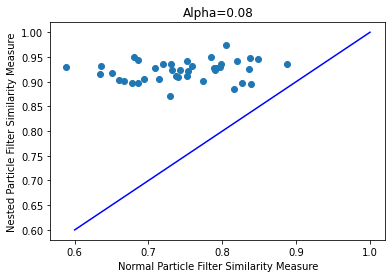
\includegraphics[scale = 0.4]{Images/synthetic_plot1.png}
    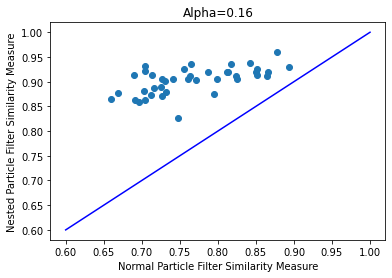
\includegraphics[scale = 0.4]{Images/synthetic_plot2.png}
    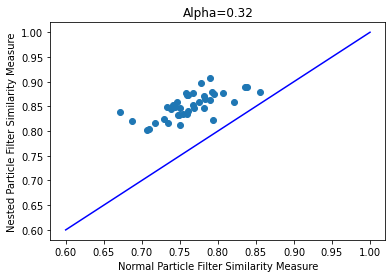
\includegraphics[scale = 0.4]{Images/synthetic_plot3.png}
    \caption{Synthetic data with different values of alpha}
\end{figure}
\begin{figure}
    \centering
    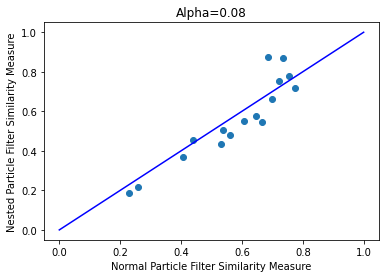
\includegraphics[scale = 0.4]{Images/human_plot1.png}
    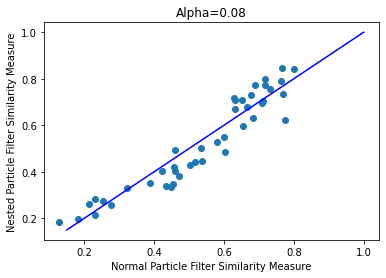
\includegraphics[scale = 0.4]{Images/human_plot2.png}
    \caption{Real data with different values of alpha} 
\end{figure}

\begin{figure}
    \centering
    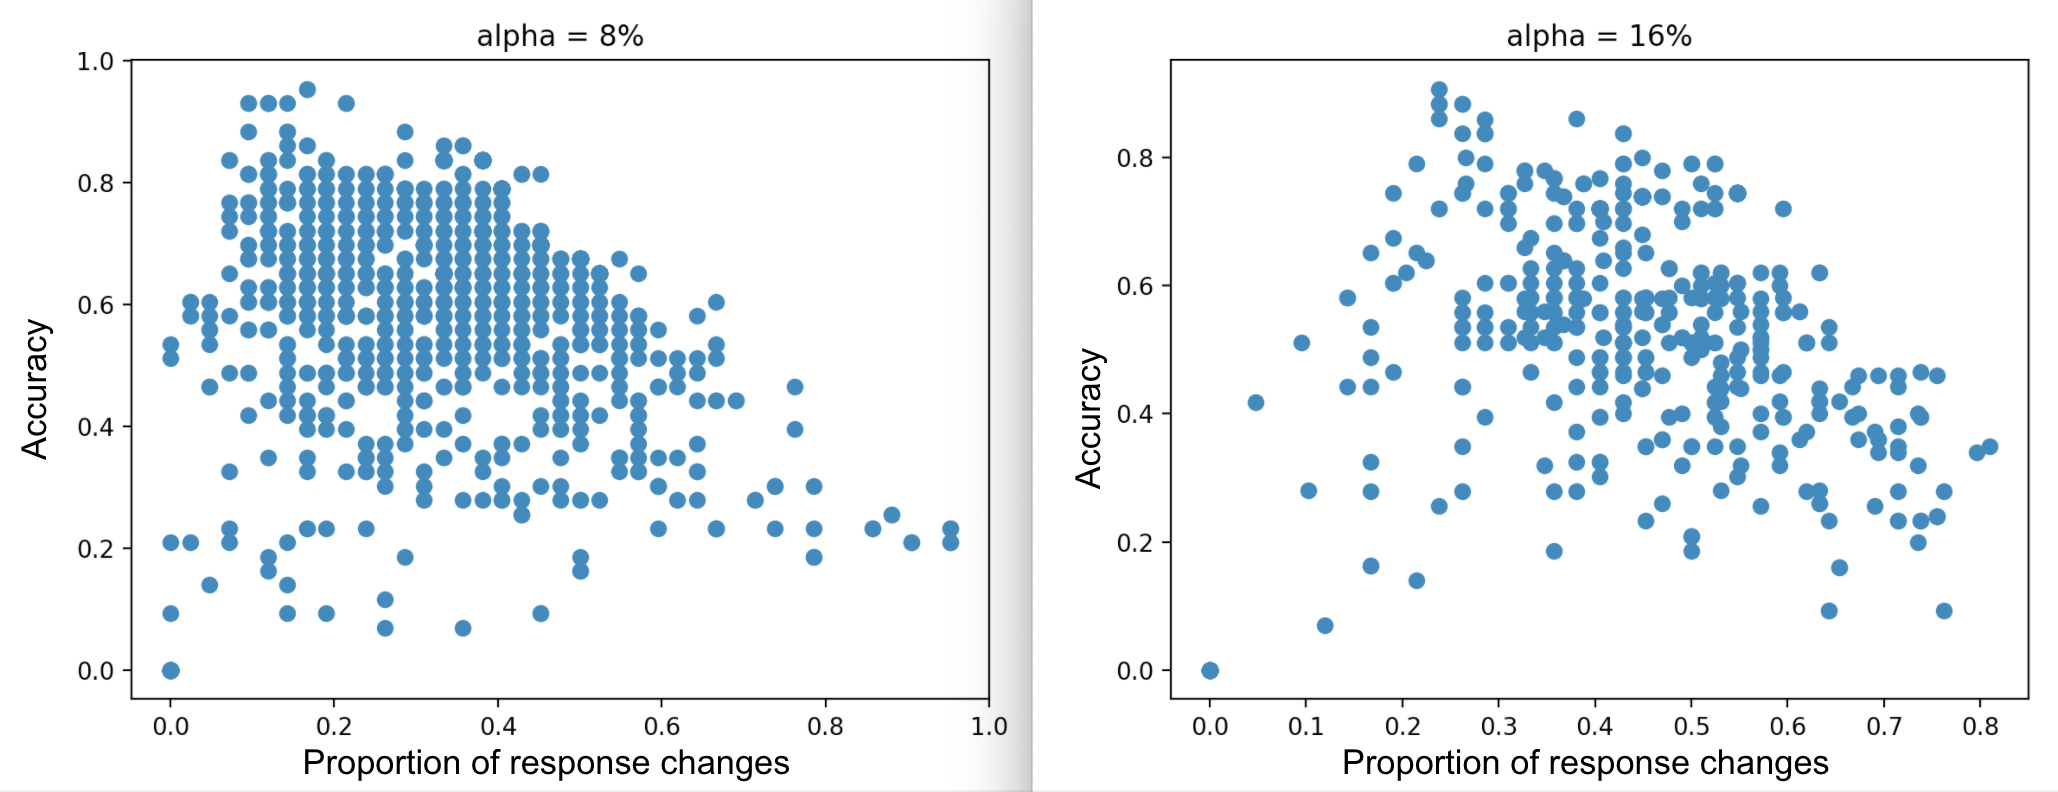
\includegraphics[scale = 0.3]{Images/Figure3.png}
    \caption{Black dots from recreated Figure 4} 
\end{figure}

\begin{figure}
    \centering
    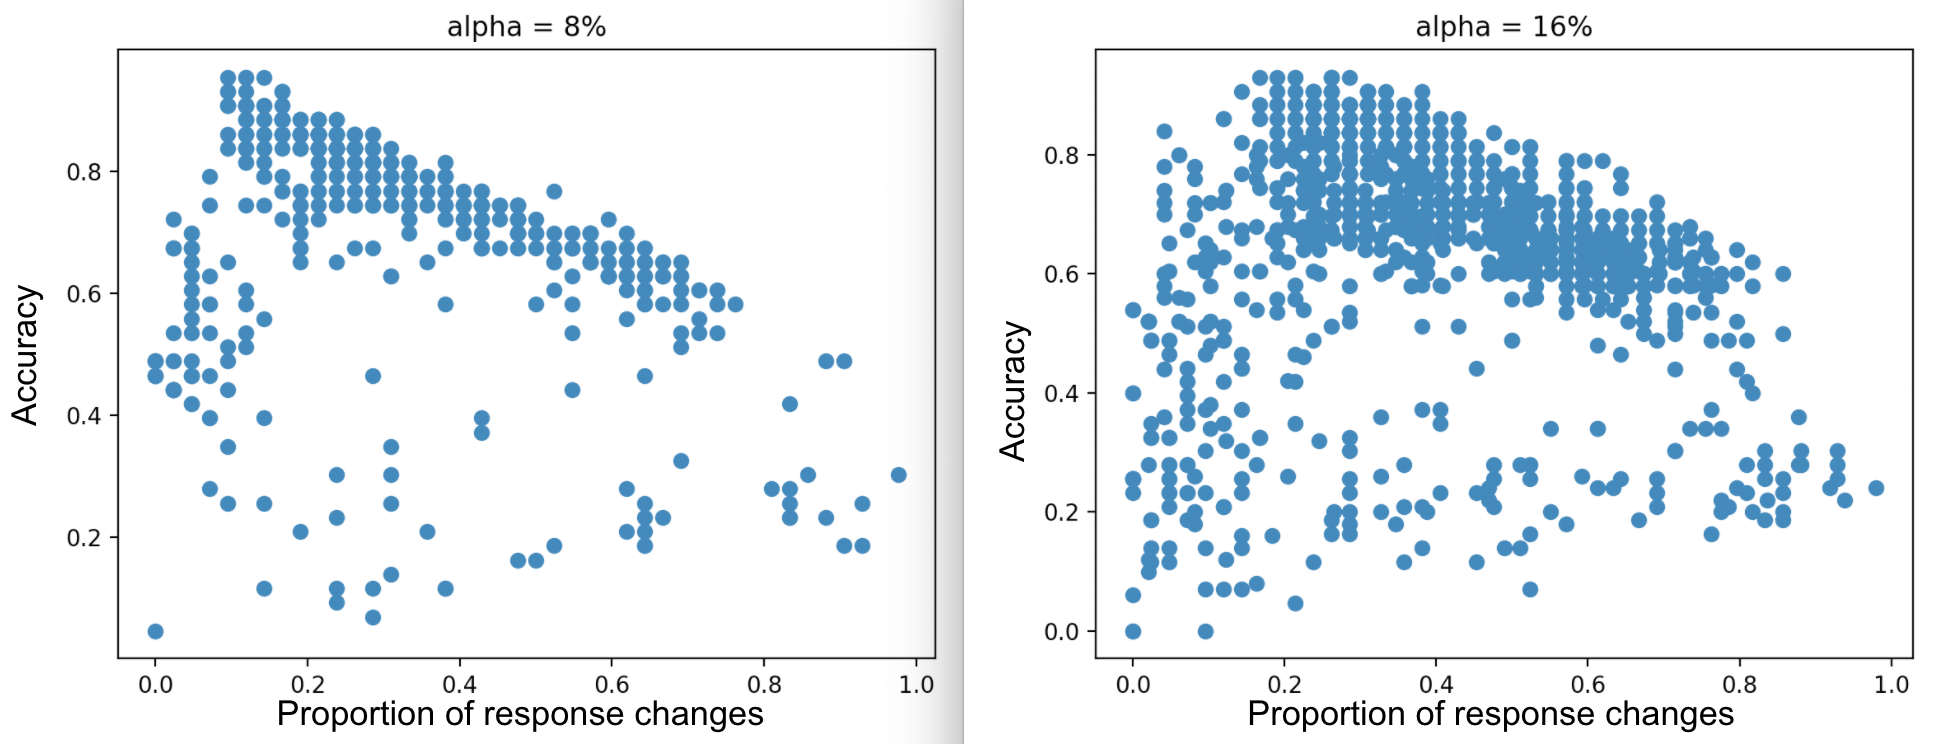
\includegraphics[scale = 0.3]{Images/Figure4.png}
    \caption{Grey dots from recreated Figure 4} 
\end{figure}

\begin{algorithm}[h!]
In the following algorithm, $S_t$ is the set of particles and weights at time $t$, $z_t$ and $u_t$ are respectively the observation and some action taken by each particle at time $t$ and $u_t$ is responsible for changing the state of the particle at time $t$
   \caption{Particle Filter Update}
    \begin{algorithmic}[1a]
      \Function\texttt{particle\_filter\_update({$S_{t-1}=\langle x_{t-1}^{j},w_{t-1}^{j}\rangle,u_t,z_t$})}
        \State $S_t = \{\}, \eta = 0$
        \For{$i = 1$ to ${n}$} \hspace{5mm} Weight Based Resampling
            \State Sample index $j(i)$ from the discrete distribution given by $w_{t-1}$ 
            \State Sample $x_{t}^i$ from $p(x_{t}|x_{t-1},u_t)$ using $x_{t}^{j(i)}$ and $u_t$
            \State $w_{t}^{i}=p(z_{t}|x_{t}^{i})$ \hspace{6mm} Compute Importance Weight(Reweight)
            \State $\eta=\eta+w_{t}^{i}$ \hspace{10mm} Update Normalization Constant
            \State $S_t = S_t \bigcup \{x_t^{i},w_t^{i}\}$
        \EndFor
        \For{$i = 1$ to ${n}$}
            \State $w_{t}^i=\frac{w_{t}^i}{\eta}$ \hspace{14mm} Normalize Weights
        \EndFor
        \State return $S_t$
        \EndFunction   
    \end{algorithmic}
\end{algorithm}

\begin{algorithm}[h!]
In the following algorithm, each nested particle filter, $P_t$ is a set of particle filters and respective weights at time $t$ and $z_t,u_t$ follows the same notation as above and $h_t$ is the human inference at time $t$, in our experimental set up this is equivalent to a state. Since each particle filter is a distribution of probability among possible states, we are introducing $S_t(s)$ as a notation which refers to the probability of a particle filter $S_t$ having state $s$
   \caption{Nested Particle Filter Update}
    \begin{algorithmic}[1]
      \Function\texttt{nested\_particle\_filter\_ update($P_{t-1}=\langle S_{t-1}^{j},w_{t-1}^{j}\rangle,u_t,z_t,h_t$)}
        \State $P'_t =\{\},\eta = 0$
        \For {$i = 1$ to ${n}$} \hspace{6mm} Updating each particle filter
            \State $S_t^i$= \texttt{particle\_filter\_update({$S_{t-1}^i,u_t,z_t$})} 
            \State $w_t^i=S_t(h_t)$
            \State $\eta = \eta + w_t^i $
            \State $P'_t = P'_t\bigcup \{S_t^i,w_t^{i}\}$
        \EndFor
        \For {$i = 1$ to ${n}$} \hspace{6mm} Normalizing weights
            \State $w_t^i=\frac{w_t^i}{\eta}$
        \EndFor
        \State $P_t=\{\}$
        \State $\eta=0$
        \For{$i = 1$ to ${n}$} \hspace{6mm} Weight Based Resampling of Partcile Filter
            \State Sample an index $j(i)$ from the discrete distribution given by $w_{t}$
            \State $P_t = P_t\bigcup \{S_t^{j(i)},w_t^{j(i)}\}$
            \State $\eta = \eta + w_t^{j(i)}$
        \EndFor
        \For {$i = 1$ to ${n}$} \hspace{6mm} Normalizing weights again after resampling 
            \State $w_t^i=\frac{w_t^i}{\eta}$
        \EndFor
    \EndFunction    
    \end{algorithmic}
\end{algorithm}

\begin{algorithm} [h!]
\texttt{state\_list=$[A,B,C,D]$}\\
$\mu = \{A:.2,B:.4,C:.6,D:.8\}$\\
$\sigma = 0.1$\\
$f(x|\sigma,\mu)={\frac {1}{\sigma {\sqrt {2\pi }}}}e^{-{\frac {1}{2}}\left({\frac {x-\mu }{\sigma }}\right)^{2}}$
\caption{Synthetic Data Generate}
\begin{algorithmic}[1a]
  \Function\texttt{synthetic\_data\_generate(observation\_list,state\_list)}
    \State \texttt{inference\_list=\{\}}
     \For {observation in \texttt{observation\_list}} 
      \State \texttt{best\_state=state\_list[0]}
       \For {state in \texttt{state\_list}}
        \If $f(\texttt{observation}|\mu[state],\sigma)>f(\texttt{observation}|\mu[\texttt{best\_state}],\sigma)$
          \State \texttt{best\_state = state}
        \EndIf
       \EndFor
        \State\texttt{inference\_list.append(best\_state)}
     \EndFor
    \State return \texttt{inference\_list}
    \EndFunction   
\end{algorithmic}
\end{algorithm}


\begin{algorithm} [h!]
$z_i$ is the pipe that the $i$th object falls from.

$y_i$ is the location that the object drops to. The subject sees only the sequence of all $y_i$

$T$ is the number of trials.

$\alpha$ is the probability that the pipe changes.

The pipes have the following locations: \{A: 0.2, B: 0.4, C: 0.6, D: 0.8\}.

\begin{verbatim}
    
1. Set z_0 to a random pipe
2. Repeat for trials i=1, …, T:
    1. Set z_i = z_{i-1} with probability 1-alpha (pipe stays the same)
       or replace z_i with a random different pipe with probability alpha
    2. Sample y_i from a normal distribution with standard deviation
       0.1 and mean of the pipe's location(z_i).

\end{verbatim}

\caption{Sequences Generate}

\end{algorithm}




\end{document}
